%%%%%%%%%%%%%%%%%%%%%%%%%%%%%% -*- Mode: Latex -*- %%%%%%%%%%%%%%%%%%%%%%%%%%%%
%% cfp.tex -- 
%% Last Modified On: Sat Jun 18 09:08:58 2016 (-0700)
%%%%%%%%%%%%%%%%%%%%%%%%%%%%%%%%%%%%%%%%%%%%%%%%%%%%%%%%%%%%%%%%%%%%%%%%%%%%%%%

\documentclass[letterpaper]{article}

\newif\ifhidelinks\hidelinkstrue
% Uncomment the next line to show hyperlinks (useful for the on-line version)
% \hidelinksfalse

\usepackage{graphicx,color,microtype}
\usepackage{tabularx}
\usepackage{hyperref}

\ifhidelinks
  \hypersetup{%
    hidelinks=true}
\else
  \hypersetup{%
    colorlinks=true,
    urlcolor=blue}
\fi

%--- Page redefinition
\usepackage{a4wide}
\setlength{\headheight}{0pt}
\setlength{\topmargin}{0pt}
\setlength{\headsep}{0pt}
\setlength{\footskip}{0pt}
\setlength{\oddsidemargin}{0pt}
\setlength{\marginparwidth}{0pt}
\setlength{\marginparsep}{0pt}
\addtolength{\textwidth}{36pt}
\hoffset-.46in
\addtolength{\textwidth}{1in}
\voffset-.5in
\addtolength{\textheight}{1.4in}
\pagestyle{empty}

%--- Macros
\definecolor{grey}{gray}{.25}
\newcommand{\affil}[1]{\enspace\textsl{\footnotesize\textcolor{grey}{#1}}}


\begin{document}

\noindent
\begin{tabularx}{\linewidth}
  {>{\small\setlength{\hsize}{.7\hsize}}X@{\quad}
    >{\setlength{\hsize}{1.3\hsize}}X}
  \vbox to0pt{\vskip-20pt\hbox to0pt{\hskip30pt
\includegraphics[width=.17\textwidth]{aflogo}\hss}\vss}
  &\centering
    {\LARGE\bfseries AFRICACRYPT~2017}\\[8pt]
  9th International Conference on the Theory and Application of\\[2pt]
  Cryptographic Techniques\par\medskip
  May 24--26, 2017\quad{\tiny$^\bullet$}\quad Dakar, Senegal
\end{tabularx}\par\vskip.3in

\noindent
\begin{tabularx}{\linewidth}
  {>{\small\setlength{\hsize}{.7\hsize}}X@{}|%
    >{\setlength{\hsize}{1.3\hsize}}X}

  \vskip.05in
  {\normalsize\bfseries Program chairs}\par\smallskip
  \begin{tabular}{l}
    Marc Joye\affil{NXP Semiconductors}\\
    Abderrahmane Nitaj\affil{Universit\'e de Caen}
  \end{tabular}\par\vskip1.5\medskipamount
  
  {\normalsize\bfseries Program committee}\par\smallskip
  \begin{tabular}{l}
    Riham Altawy\affil{Concordia University}\\
    Abdelhak Azhari\affil{Universit\'e de Casablanca}\\
    Hussain Benazza\affil{Universit\'e Moulay Ismail}\\
    Dario Catalano\affil{Universita di Catania}\\
    Pierre-Louis Cayrel\affil{Univ. Saint Etienne}\\
    Sherman S.M. Chow\affil{CU Hong Kong}\\
    Nadia El Mrabet\affil{EMSE}\\
    Pierre-Alain Fouque\affil{Universit\'e Rennes I}\\
    Jens Groth\affil{University College London}\\
    Javier Herranz\affil{U.\@ Polit\`ecnica de Catalunya}\\
    Tetsu Iwata\affil{Nagoya University}\\
    Saqib Kakvi\affil{University of Bristol}\\
    Seny Kamara\affil{Brown University}\\
    Fabien Laguillaumie\affil{Universit\'e de Lyon I}\\
    Beno\^{\i}t Libert\affil{ENS Lyon}\\
    Mark Manulis\affil{University of Surrey}\\
    Tarik Moataz\affil{Colorado State University}\\
    Ayoub Otmani\affil{Universit\'e de Rouen}\\
    Vanishree Rao\affil{PARC}\\
    Tajje-eddine Rachidi\affil{Al Akhawayn Univ.}\\
    Magdy Saeb\affil{Arab Academy for Science}\\
    Rei Safavi-Naini\affil{University of Calgary}\\
    Kazue Sako\affil{NEC}\\
    Palash Sarkar\affil{Indian Statistical Institute}\\
    Peter Schwabe\affil{Radboud Universiteit}\\
    Francesco Sica\affil{Nazarbayev University}\\
    Djiby Sow\affil{Universit\'e de Dakar}\\
    Willy Susilo\affil{University of Wollongong}\\
    Christine Swart\affil{Univ. Cape Town}\\
    Fran\c{c}ois-Xavier Standaert \affil{UCL}\\
    Joseph Tonien\affil{University of Wollongong}\\
    Amr M. Youssef\affil{Concordia University}
  \end{tabular}\par\vskip1.5\medskipamount

  {\normalsize\bfseries General chairs}\par\medskip
  \begin{tabular}{l}
    Mamadou Sanghar\'e\affil{Universit\'e de Dakar}\\
    Djiby Sow\affil{Universit\'e de Dakar}\\
    Abdoul Aziz Ciss\affil{Polytechnique Thies}
  \end{tabular}\par\vskip.4in

  \vbox to0pt{\hbox to0pt{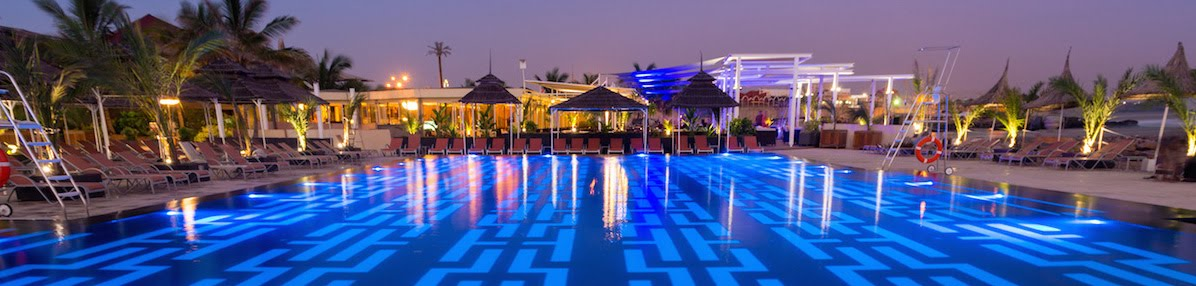
\includegraphics[width=.32\textwidth]{afvenue}\hss}\vss}\par\vskip.5in
  {\scriptsize\textcolor{grey}{\slshape Terrou-Bi Hotel, Dakar, Senegal}}\par\vskip.2in
  {\normalsize\bfseries Important dates}\par\smallskip
  \begin{tabular}{l}
    Submission deadline: \underline{\smash{\bfseries January 15, 2017}}\\
    Notification: February 28, 2017\\
    Camera-ready version: March 10, 2017\\
    Conference dates: May 24--26, 2017
  \end{tabular}
& 
  Africacrypt is an Annual International Conference on the Theory and
  Application of Cryptology. Africacrypt 2017 is organized by Cheikh
  Anta Diop University, Dakar, Senegal, in cooperation with the International
  Association for Cryptologic Research (IACR). The aim of
  Africacrypt 2017 is to provide an international forum for
  practitioners and researchers from industry, academia and
  government from all over the world for a wide ranging discussion
  of all forms of cryptography and its applications.\par\bigskip

  The program committee is seeking original research papers pertaining
  to all aspects of cryptography as well as tutorials are
  solicited. Submissions may present theory, techniques, applications
  and practical experience on topics including, but not limited
  to:\par\medskip {\small\hskip.5em 
  \begin{tabular}{l@{~}p{.915\hsize}}
    --&  Secret-key cryptography (block ciphers, stream ciphers, hash
        functions, MAC, \dots);\\ 
    --&  Secret-key cryptanalysis;\\
    --&  Public-key cryptography (identification protocols, digital
        signatures, encryption, \dots);\\ 
    --&  Public-key cryptanalysis;\\
    --&  Cryptographic protocols;\\
    --&  Design of cryptographic schemes;\\
    --&  Security proofs;\\
    --&  Anonymity (electronic commerce and payment, electronic voting, \dots);\\
    --&  Information theory;\\
    --&  Foundations and complexity theory;\\
    --&  Multi-party computation;\\
    --&  Quantum cryptography;\\
    --&  Elliptic curves;\\
    --&  Lattices;\\
    --&  Code-based cryptography;\\
    --&  Efficient implementations.\\
  \end{tabular}}


  \section*{Instructions for authors}

  Authors are invited to submit papers (PDF format) with novel
  contributions electronically using the submission form available on
  the conference web site.
  Submitted papers must be original, unpublished, \emph{anonymous},
  and not submitted to journals or other conferences/workshops that
  have proceedings. Submissions must be written in English and should
  be at most 18 pages in total including bibliography and
  appendices. Papers not meeting these guidelines risk rejection
  without consideration. All submissions will be
  blind-refereed.\par\smallskip

  Authors of accepted papers must guarantee that their
  paper will be presented at the conference and must make a full
  version of their paper available online.\par\bigskip  

  For submission instructions and further
  information please point your web-browser to:
  \begin{center}
    \url{https://sites.google.com/site/africacrypt2017/}
  \end{center}
  
  \section*{Proceedings}
  The proceedings will be published in the Springer Lecture Notes in
  Computer Science (LNCS) series. Accepted papers should follow the
  \href{https://www.springer.com/computer/lncs?SGWID=0-164-6-793341-0}{LNCS default author instructions}. 
\end{tabularx}

\end{document}
